\chapter{Конструкторская часть}

В данном разделе разработаны схемы реализаций алгоритма выделения наиболее информативных терминов из выборки документов.

\section{Разработка алгоритмов}

На рисунках \ref{fig:tf} -- \ref{fig:thread_work} приведены схемы однопоточной и многопоточной реализаций рассматриваемого алгоритма.

\begin{figure}[h]
	\centering
	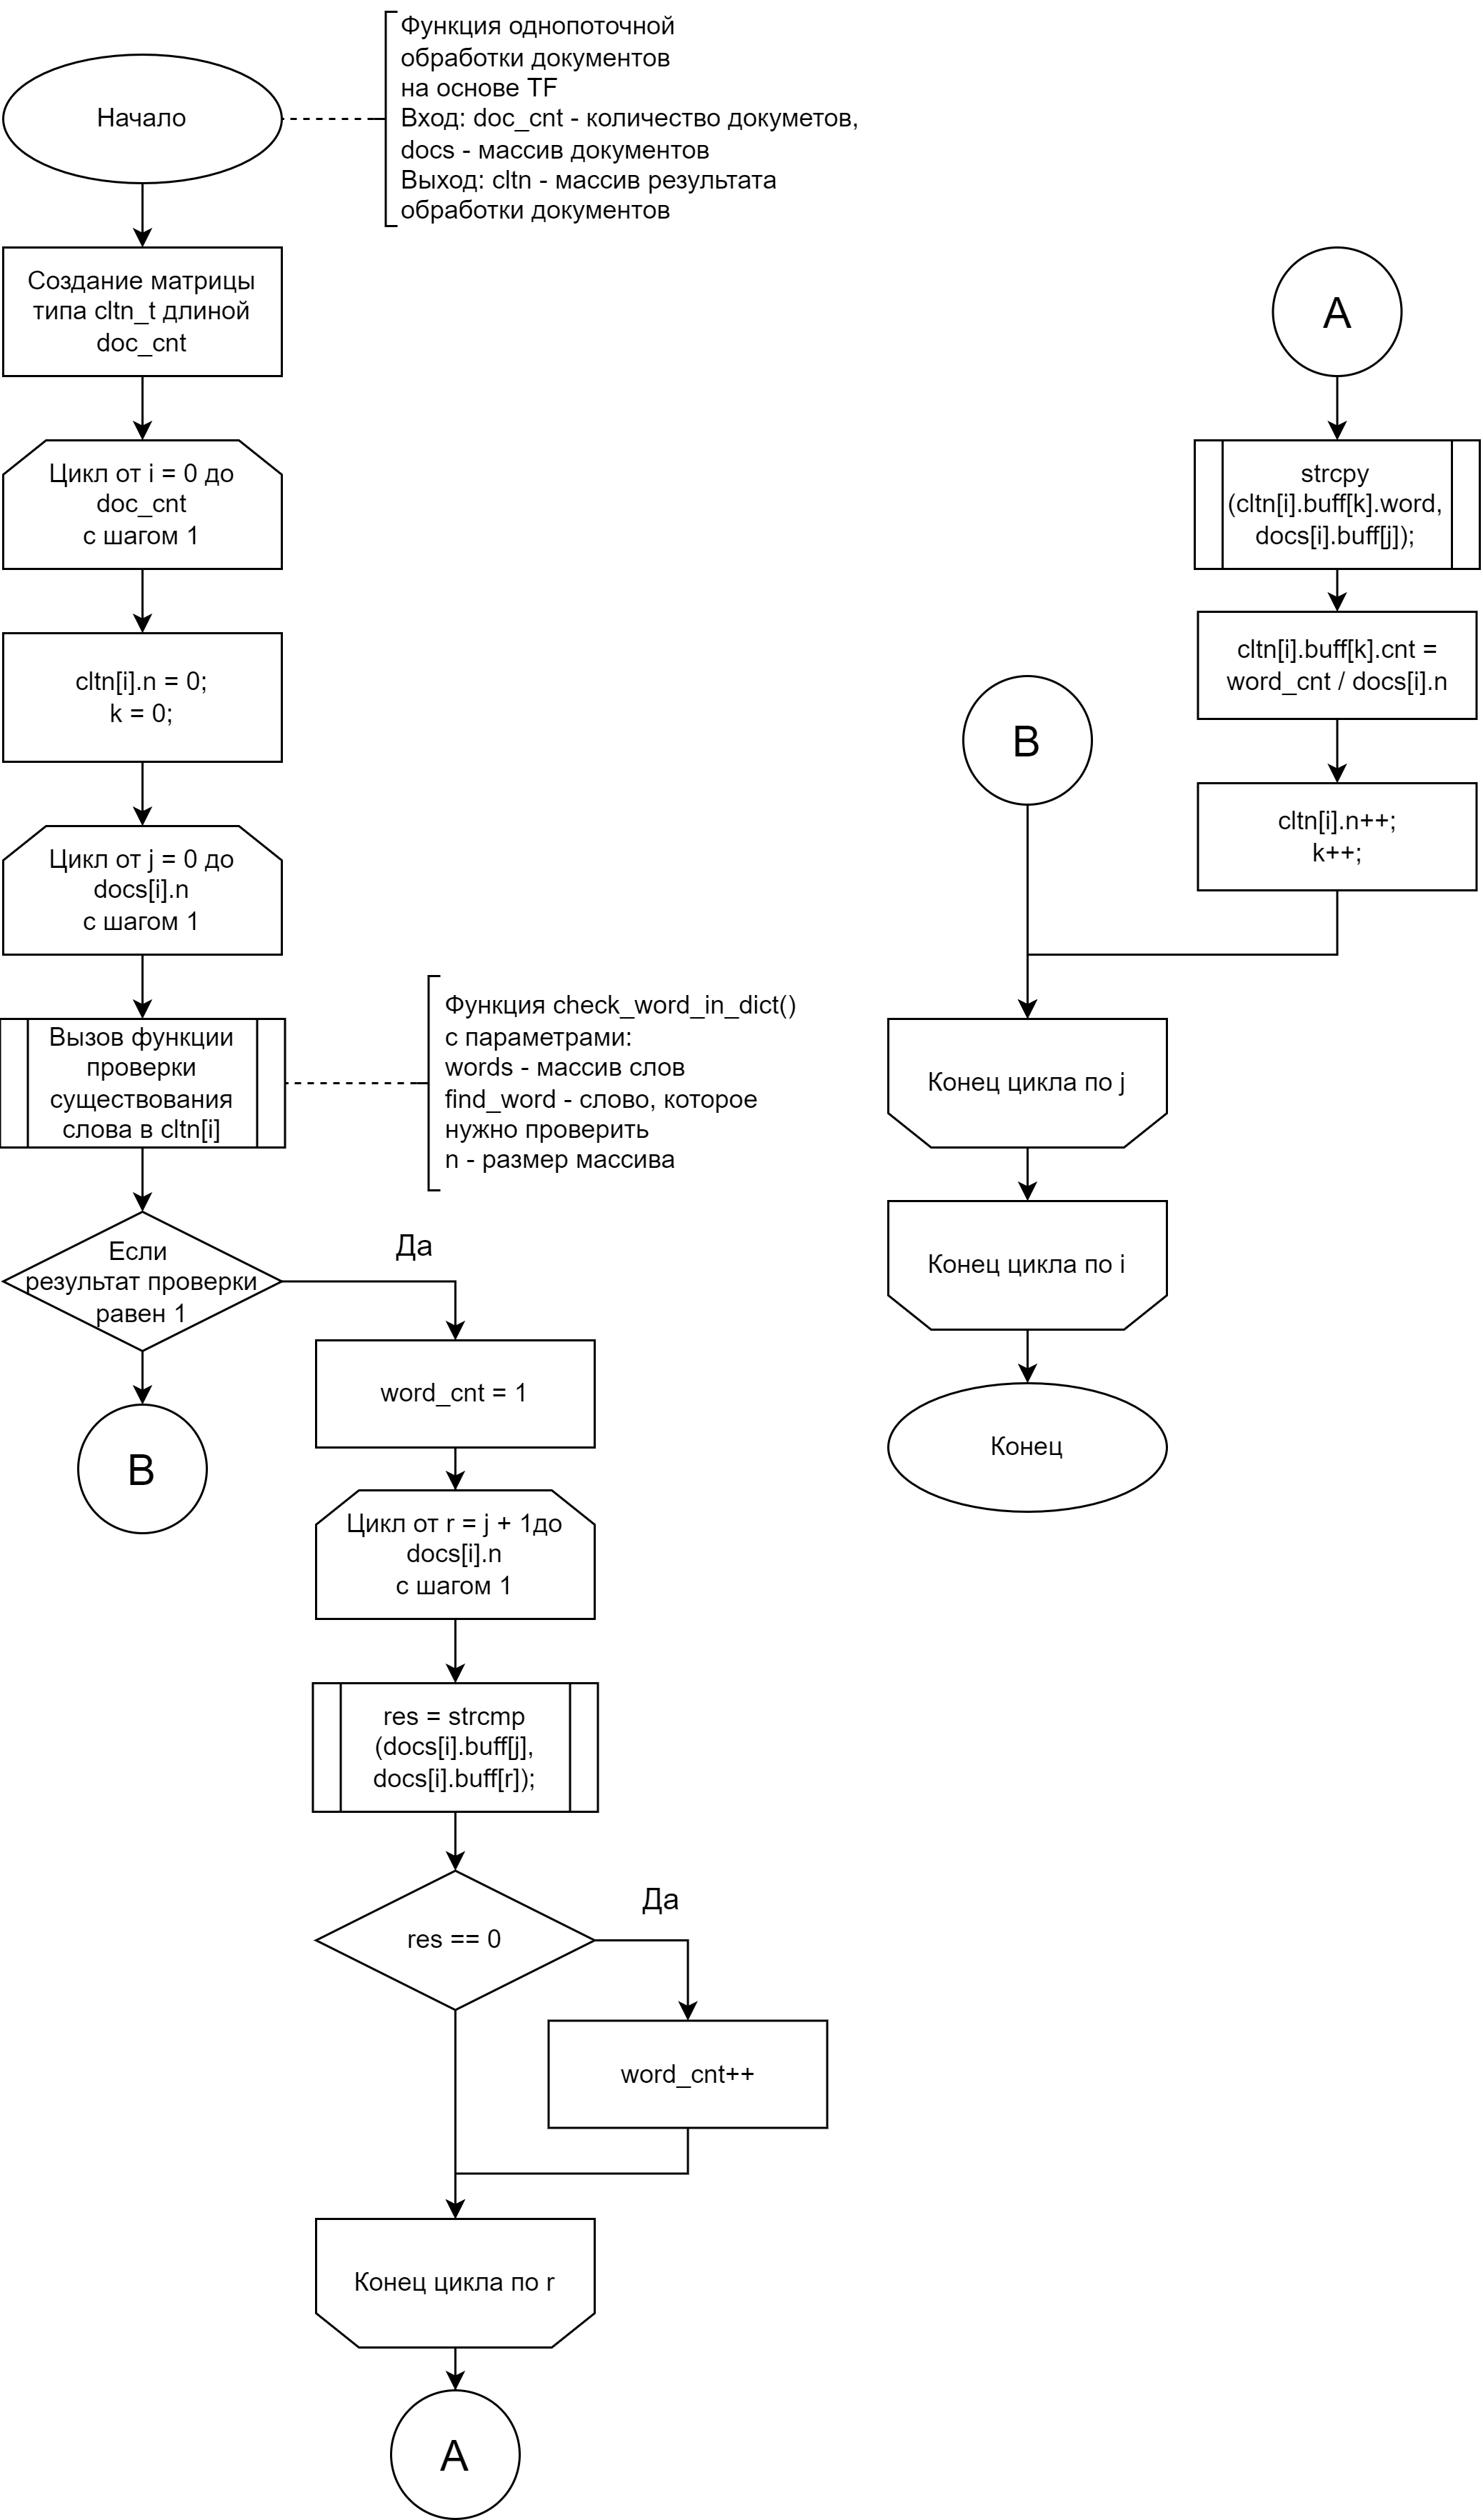
\includegraphics[width=0.85\textwidth]{img/tf_alg.png}
	\caption{Схема однопоточного алгоритма выделения терминов из выборки документов на основе частоты термина}
	\label{fig:tf}
\end{figure}

\clearpage

\begin{figure}[h]
	\centering
	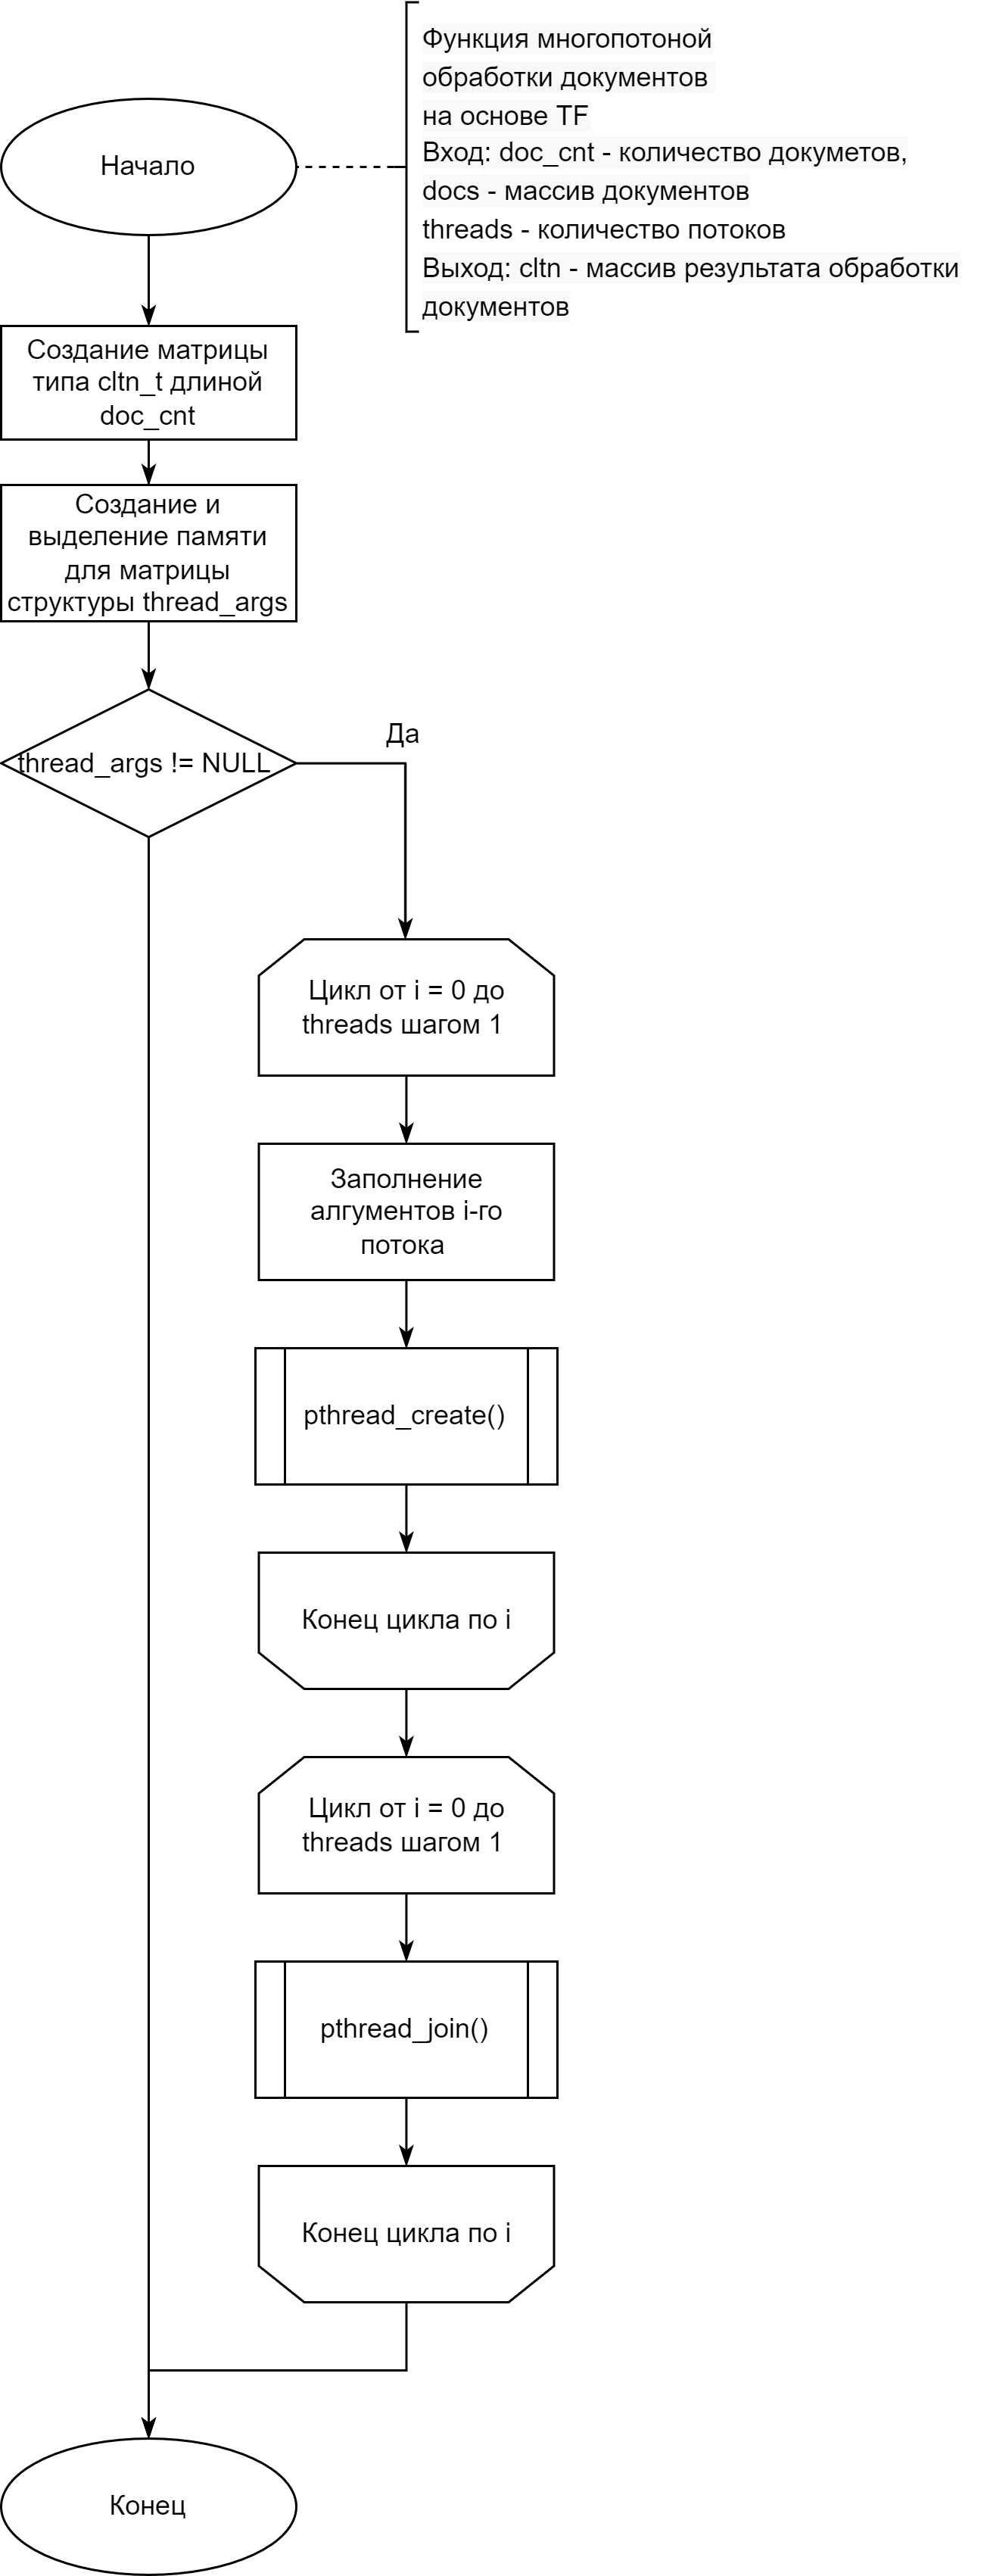
\includegraphics[height=0.85\textheight]{img/parallel.png}
	\caption{Схема алгоритма работы основного потока, запускающего вспомогательные потоки}
	\label{fig:parallel}
\end{figure}

\clearpage

\begin{figure}[h]
	\centering
	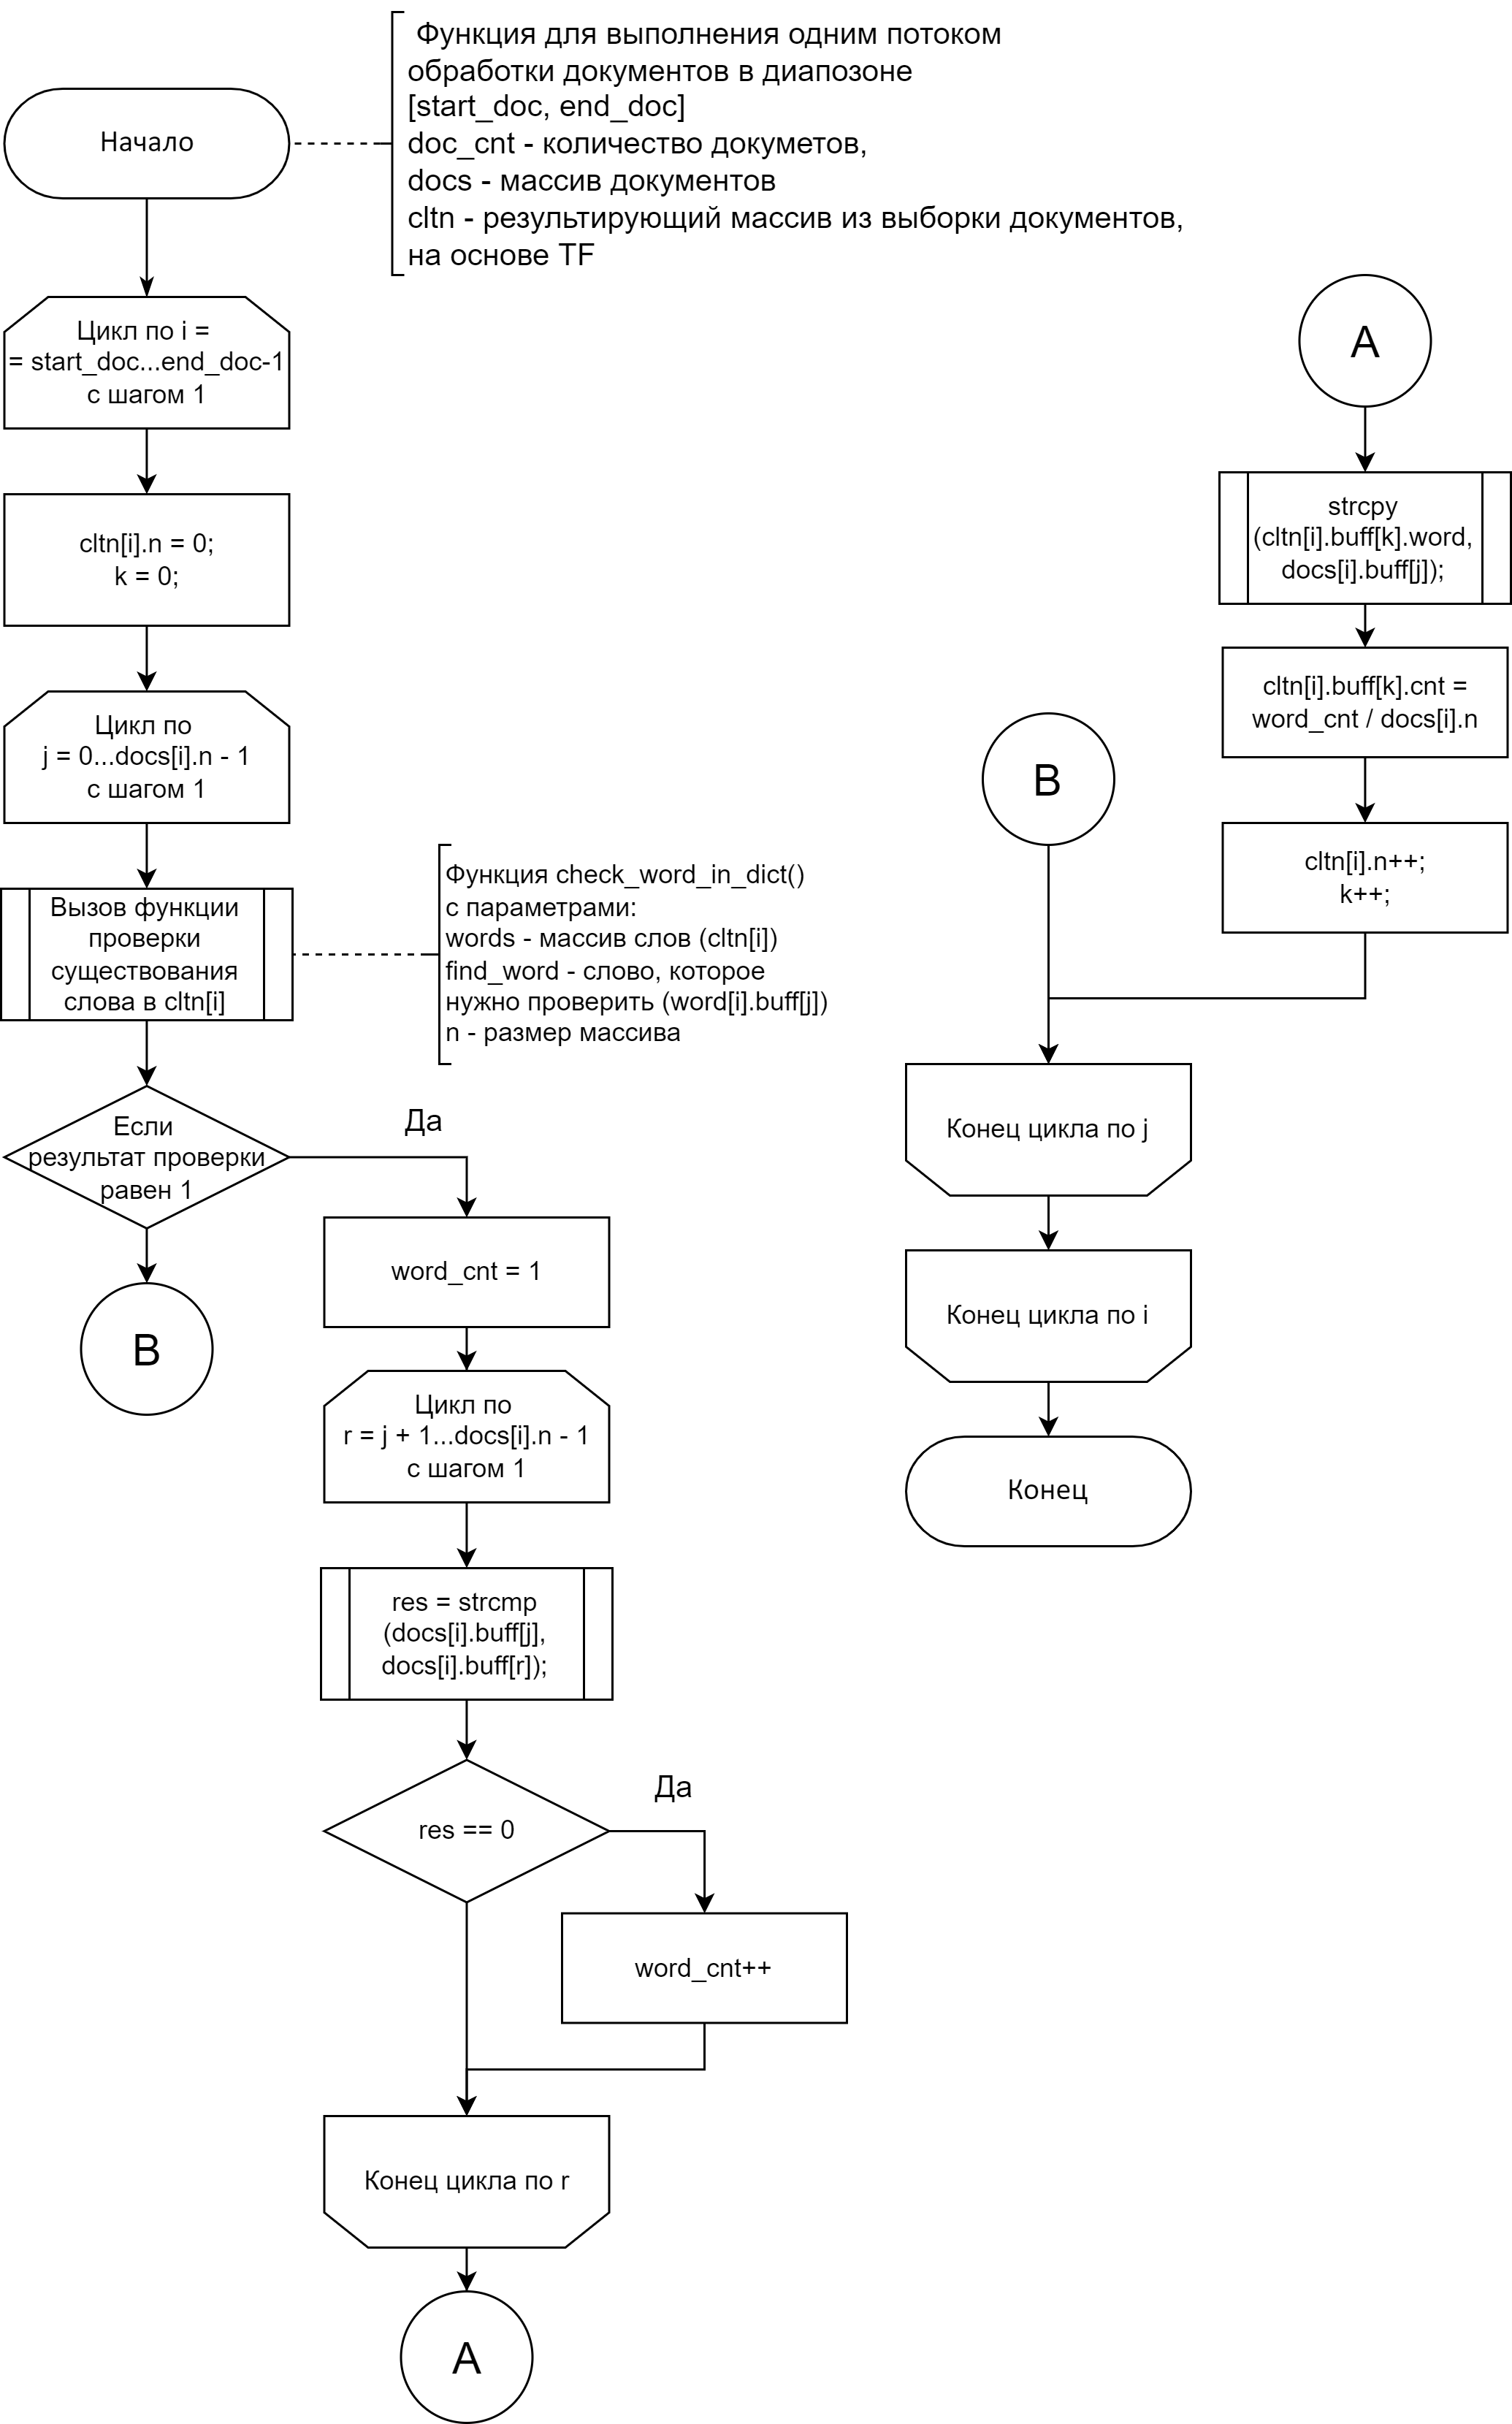
\includegraphics[height=0.85\textheight]{img/thread_work.png}
	\caption{Схема однопоточного алгоритма выделения терминов из выборки документов на основе частоты термина}
	\label{fig:thread_work}
\end{figure}

\clearpage

\begin{figure}[h]
	\centering
	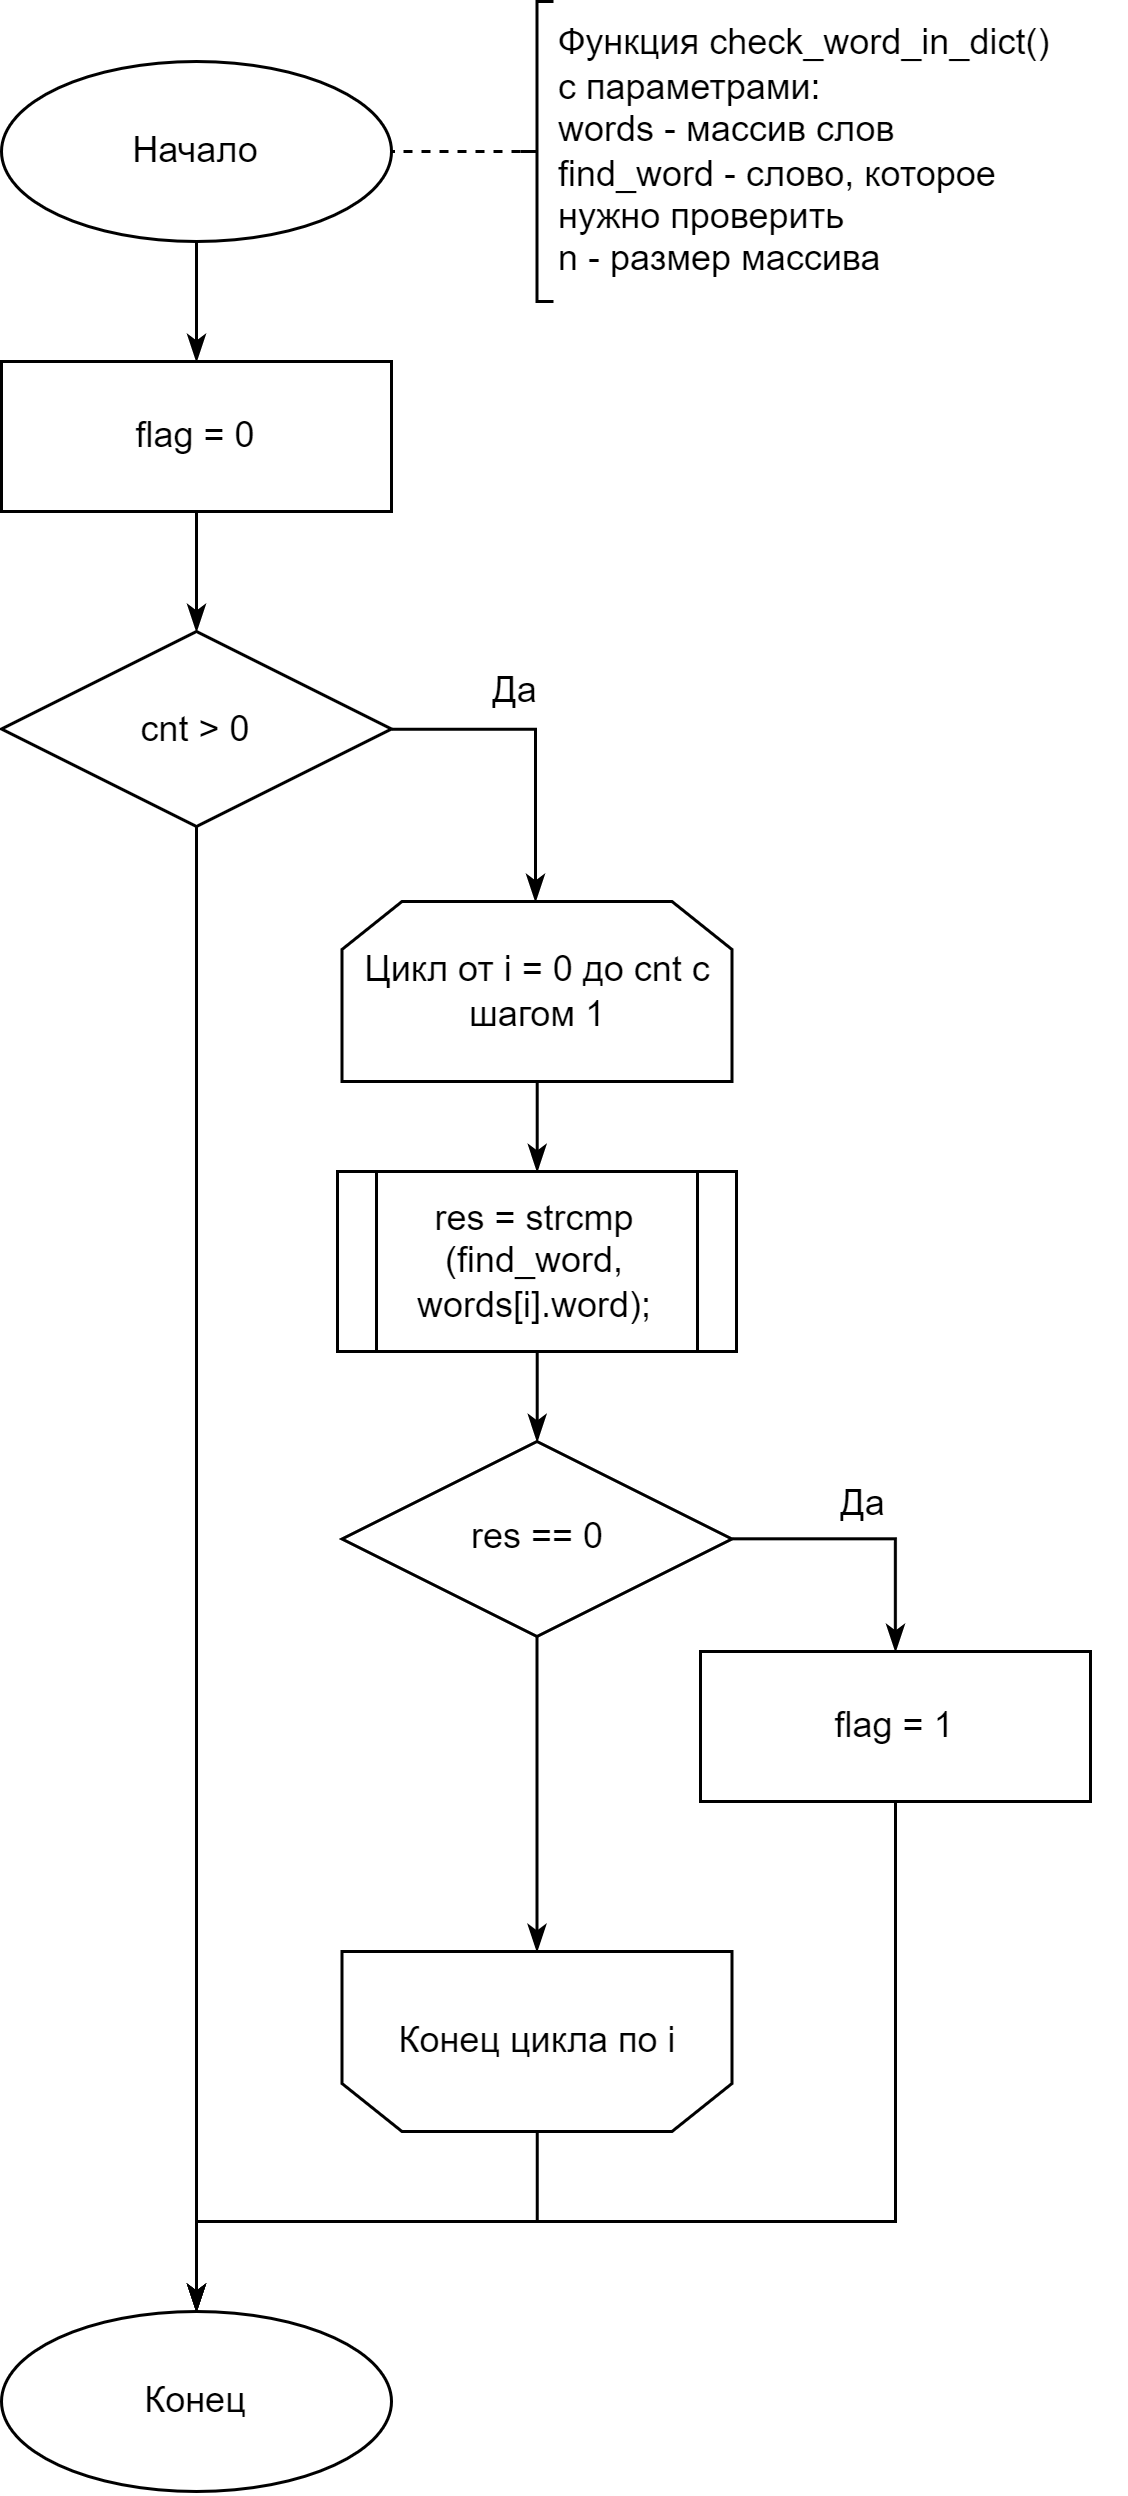
\includegraphics[height=0.7\textheight]{img/check_word.png}
	\caption{Схема алгоритма проверки существования слова в массиве}
	\label{fig:check}
\end{figure}

\section*{Вывод}

В данном разделе разработаны схемы реализаций рассматриваемого алгоритма